%%%%%%%%%%%%%%%%%%%%%%%%%%%%%%%%%%%%%%%%%
% Beamer Presentation
% LaTeX Template
% Version 1.0 (10/11/12)
%
% This template has been downloaded from:
% http://www.LaTeXTemplates.com
%
% License:
% CC BY-NC-SA 3.0 (http://creativecommons.org/licenses/by-nc-sa/3.0/)
%
%%%%%%%%%%%%%%%%%%%%%%%%%%%%%%%%%%%%%%%%%

%----------------------------------------------------------------------------------------
%	PACKAGES AND THEMES
%----------------------------------------------------------------------------------------

\documentclass{beamer}

\mode<presentation> {
\usetheme{default} %
\usecolortheme{seagull} 
}

\usepackage{graphicx} % Allows including images
\usepackage{booktabs} % Allows the use of \toprule, \midrule and \bottomrule in tables
\usepackage{tipa}
\usepackage[T1]{fontenc}
\usepackage{tikz}
\usepackage{tabularx}
	\newcolumntype{L}{>{\raggedright\arraybackslash}X}

\usepackage{multirow}
\usepackage{hyperref}
\hypersetup{
    colorlinks=true,   
    urlcolor=blue,
}
%\href{<url>}{<text to display>}

\pgfdeclareimage[width=\paperwidth]{mybackground}{MelSpecfrench35.png}
%----------------------------------------------------------------------------------------
%	TITLE PAGE
%----------------------------------------------------------------------------------------
\title[Audio Language Classifier]{Audio Language Classifier} % The short title appears at the bottom of every slide, the full title is only on the title page
\author{Kirsten Regier} % Your name
\date{December 20, 2020} % Date, can be changed to a custom date
%----------------------------------------------------------------------------------------

\begin{document}

\begin{frame}
\titlepage % Print the title page as the first slide
\end{frame}

%----------------------------------------------------------------------------------------
%	PRESENTATION SLIDES
%----------------------------------------------------------------------------------------
%------------------------------------------------
\section{Problem Statement} % 1-2 slides
%------------------------------------------------
\begin{frame}
\frametitle{Why Audio Classifiers?}

\textbf{Goal}: Using the VGGish model as a feature extractor, build and train a classifier to identify speaker characteristics (gender or native language) from audio files.
\vspace{1em}

Automatic speech recognition (ASR) and voice assistants are expanding.
\vspace{1em}

ASR systems don't work well with non-standard or non-native accents \cite{Sheng}.
\vspace{1em}

Better speech technology may improve customer experiences and customer service.
%Deep learning can provide acoustic insights that are difficult to attain through mathematical and physics-based methods (Bianco, et. al, 2019).
\end{frame}
%------------------------------------------------
\section{The Data} % 1 slide
%------------------------------------------------
\begin{frame}
\frametitle{The Data}

\href{https://www.kaggle.com/rtatman/speech-accent-archive}{Speech Accent Archive} \cite{Weinberger}

\begin{itemize}
\item 2000+ recordings of speech samples.
\item Speakers read a fixed passage in English.
\item Demographic information about speakers: age, sex, birthplace, country, native language.
\begin{itemize}
\item Speakers from 177 countries.
\item Native speakers of 199 native languages.
\item 78 languages represented by a single speaker.
\item 121 languages with multiple speakers.
\end{itemize}
\end{itemize}

\end{frame}
%------------------------------------------------
\begin{frame} 
\frametitle{Distribution of Speakers by Gender}
\begin{center}
\begin{figure}
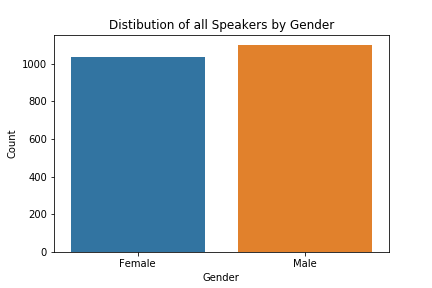
\includegraphics[width=4.25in]{GenderDistAll.png}
\end{figure}
\end{center}
\end{frame}
%------------------------------------------------
\begin{frame} 
\frametitle{Top 10 Languages in Speech Accent Archive}

\begin{center}
\begin{figure}
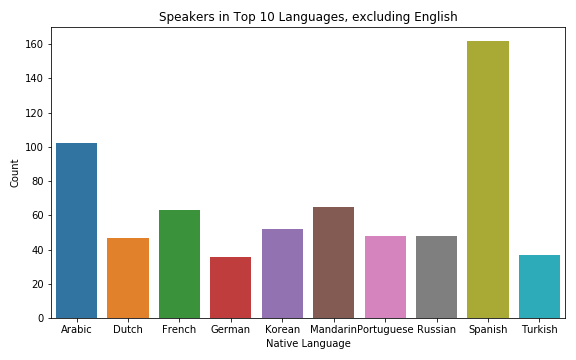
\includegraphics[width=4.25in]{TopLangCount.png}
\caption{Number of speakers for top 10 languages, excluding English}
\end{figure}
\end{center}

\end{frame}


%------------------------------------------------
\section{Hypothesis} % 3-4 slides
%------------------------------------------------
\begin{frame}
\frametitle{Transfer Learning}

%What is transfer learning?
%\begin{itemize}
%\item Reuse parts of a network that has already been trained on a large dataset as the basis for a new model (Bianco, et. al. 2019)
%\end{itemize}

%\vspace{1em}
Transfer learning from image classification models has been an effective starting point for audio classification. \cite{Hershey}
\vspace{1em}

 \href{https://github.com/tensorflow/models/tree/master/research/audioset/vggish}{VGGish} is an audio embedding model based on the architecture of the VGG image classifier, that has been trained on the \href{https://research.google.com/youtube8m/}{YouTube-8M Segments Dataset} for Acoustic Event Detection Classification (AED). \cite{Hershey}
\vspace{1em}

Features extracted by VGGish for AED may be useful for training models for (acoustic) speech classification, with relatively short training times and small datasets.

% available from \href{https://github.com/tensorflow/models/tree/master/research/audioset/vggish}{GitHub} and \href{https://tfhub.dev/google/vggish/1}{Tensorflow Hub}

%\begin{block}{Benefits}
%\begin{itemize}
%\item Reduced training time for new models.
%\item New models can use smaller datasets.
%\item Generalized features feed into customized classification layers.
%\item Possible to fine-tune the entire model after convergence of new elements.
%\end{itemize}
%\end{block}

\end{frame}
%------------------------------------------------
\section{Modeling} % 3-4 slides
%------------------------------------------------
\begin{frame}
\frametitle{Model Architecture}

Audio files fed through the VGGish model.
\begin{itemize}
\item Audio segment (10s) converted to mel spectrogram.
\item Mel spectrogram fed through VGGish convolutional layers.
\item VGGish output is a 128-D array of features.
\end{itemize}
\vspace{1em}
%All classifier models contain
%\begin{itemize}
%\item Input layer - (Batch size, 10, 128)
%\item Dense, fully connected layer, variable number of nodes
%\item 50\% Dropout layer 
%\item 1-D Flatten layer - size based on output of previous layer
%\item Output layer - (Batch size, Number of classes)
%\end{itemize}

VGGish features fed to a Gender Classifier or a Language Classifier.
\vspace{1em}

Classifier models vary in:
\begin{itemize}
\item Number of (Dense + Dropout) layer repeats.
\item Number of nodes in Dense layer(s).
\item Shape of Flatten layer (based on output of previous layer)
\end{itemize}

\end{frame}
%------------------------------------------------
\begin{frame}
\frametitle{Gender Classifier Architecture}

\begin{table}[!h]
\begin{center}
\caption{Structure of the Gender Classifier models.}
\begin{tabular}{l | c | c |}
Layer  & Gender 1 & Gender 2\\
\hline

Input 	& (32, 10, 128) & (32, 10, 128) \\ \hline

Dense	& 128 nodes & 128 nodes \\
Dropout	& 50\%		& 50 \% \\ \hline

Dense	&			& 64 nodes \\
Dropout	& 			& 50\% \\ \hline

Flatten 	& (32, 1280)	& (32, 640) \\ \hline
Output 	& (32, 1)		& (32, 1)\\
\hline
\end{tabular}

\label{tab:GenModels}
\end{center}
\end{table}
%\end{block}
\end{frame}
%------------------------------------------------
\begin{frame} 
\frametitle{Language Classifier Architecture}

\begin{table}[!h]
\begin{center}
\caption{Structure of the Language Classifier models.}
\begin{tabular}{l | c |c  | c |}

Layer  & Language 1 & Language 2 & Language 3\\
\hline

Input 	& (32, 10, 128)& (32, 10, 128) & (32, 10, 128) \\ \hline

Dense	& 12 nodes 	& 128 nodes 	& 128 nodes \\
Dropout	& 50\%		& 50\%		& 50 \% \\ \hline

Dense	&			&			& 64 nodes \\
Dropout	&			& 			& 50\% \\ \hline

Flatten 	& (32, 120)	& (32, 1280)	& (32, 640) \\ \hline
Output 	& (32, 11)		& (32, 11)		& (32, 11)\\
\hline
\end{tabular}

\end{center}
\end{table}
\end{frame}
%------------------------------------------------
\section{Modeling Results and Analysis } % 3-4 slides
%------------------------------------------------
\begin{frame}
\frametitle{Results}

\begin{block}{Gender Classifier}
Identify the gender of the speaker.
\begin{itemize}
\item Convergence after 2-3 epochs.
\item 98\% accuracy.
\end{itemize}
\end{block}

\begin{block}{Language Classifier}
Identify the native language of the speaker.
\begin{itemize}
\item 11 language classes.
\item Convergence after 7 epochs.
\item 25\% accuracy with majority class distribution of 15\%.
\end{itemize}
\end{block}

\end{frame}
%------------------------------------------------
%------------------------------------------------
\begin{frame}
\frametitle{Gender Classifiers - Model Metrics}

\begin{table}[h]
\begin{center}
\caption{Summary Metrics}
\begin{tabular}{l c c}
& 	Gender 1 & Gender 2 \\ \hline
Loss	&0.061640 & 0.076962 \\
Accuracy& 0.981419 & 0.975507 \\
Precision & 0.982818 & 0.960199 \\
Recall & 0.979452 & 0.991438 \\
\end{tabular}

\begin{table}
\begin{center}
\caption{Confusion Matrices}
\begin{tabular}{l r | c c l r |c c }
& & \multicolumn{2}{c}{Predicted} & & & \multicolumn{2}{c}{Predicted}  \\
\textbf{Gender 1}  & & F & M  & & \textbf{Gender 2} & F & M \\ \hline
\multirow{2}{*}{Actual} & F & 590 &  10 &  & F& 576 &  24\\
& M & 12 & 572 & & M &  5 & 579 \\
\end{tabular}
\end{center}
\end{table}

%\label{tab:GenMetricsSum}
\end{center}
\end{table} 
\end{frame}
%-----------------------------------------------
\begin{frame}
\frametitle{Language Classifier - Model Metrics}

11 language classes.
\vspace{1em}

Baseline accuracy of 15\% based on majority class distribution.

\begin{table}[h]
\begin{center}
%\caption{Language Classifiers - Metrics summary}
\begin{tabular}{l l c c c}
& 			& Language 1	& Language 2	& Language 3\\ \hline
&Loss		&2.25485		&2.323		&2.20684 \\
&Accuracy	&0.232955	&0.238636	&0.25\\
&Precision	&0.625		&0.5			&0.605263\\
&Recall	&0.0142045	&0.0738636	&0.0653 \\  \hline
\multirow{3}{*}{F1 score} & Micro	&0.232955	&0.238636	&0.25\\
&Macro	&0.16999		&0.195512	&0.191103\\
&Weighted	&0.20067	&0.228178	&0.224565\\
\end{tabular}
%\label{tab:LangMetricsSum}
\end{center}
\end{table} 

\end{frame}
%------------------------------------------------
\begin{frame} 
\frametitle{Language Classifier - Confusion Matrix}

\begin{footnotesize}
\begin{table}
\begin{center}
\caption{Confusion matrix for Language 3 predictions. The bold numbers on the diagonal represent correct predictions.}
\begin{tabular}{l | c c c c c c c c c c c || c}
lang			&R &A &T &K &G &D &S &F &E &P &M & Segments\\ \hline
Russian		&\textbf{0}  &2  &1  &4  &0  &1  &7  &4  &1  &1  &7 &28\\
Arabic		&0 &\textbf{24}  &0  &4  &1  &7  &2  &2  &4  &0 &11 &55\\
Turkish		&0  &1  &\textbf{1}  &4  &0  &3  &4  &0   &2  &1  &5 &21\\
Korean		&1 &10  &0  &\textbf{6}  &0  &3  &2  &2  &4  &2  &1 &31\\
German		&0  &0  &0  &1  &\textbf{0}  &0  &5  &1  &5  &2  &1 &15\\
Dutch		&0  &4  &0  &0  &0 &\textbf{12} & 3  &1  &3  &1  &1 &25\\
Spanish		&1  &2  &0  &6  &2  &1 &\textbf{12}  &3  &8  &0  &7 &42\\
French		&1  &3  &0  &4  &1  &2 &10 & \textbf{5}  &1  &1  &4 &32\\
English		&0  &1  &0  &3  &0  &5  &2  &2 &\textbf{13}  &0  &4 &30\\
Portuguese	&0  &3  &0  &3  &1  &0  &7  &5  &3  &\textbf{0}  &6 &28\\
Mandarin		&0  &2 & 0  &8  &2  &4  &9  &1  &2  &2 &\textbf{15} &45\\ \hline
Total			&3 &52 &2 &43 &7 &38 &63 &26 &46 &10 &62 &\textbf{352}\\

\end{tabular}
\label{tab:LangConfMat}
\end{center}
\end{table}

\end{footnotesize}

\end{frame}

%------------------------------------------------
\section{Summary \& Conclusions} % 1 slide
%------------------------------------------------
%------------------------------------------------
\begin{frame} 
\frametitle{Conclusions}

\begin{itemize}
\item Transfer learning is an effective strategy for training speech models.
\item Acoustic features extracted by VGGish for AED are adequate to train a gender classifier with 98\% accuracy.
\item Language classifier with 11 classes shows improvement over majority class baseline.
\end{itemize}

\textbf{Future directions}: Optimize language classifier.
\begin{itemize}
\item Add more layers and/or nodes.
\item Use different activation functions.
\item Include additional acoustic features (e.g. tempo/beat tracking).
\end{itemize}

\end{frame}
%------------------------------------------------
\begin{frame} 
\frametitle{References}

\scriptsize{
\begin{thebibliography}{99} % does not support BibTeX so references must be inserted manually as below
\bibitem[Tensorflow]{TF} Abadi, M., Agarwal, A., Barham, P., Brevdo, E., Chen, Z., Citro, C., Corrado, G. S.,  Davis,  A.,  Dean, J.,  Devin, M.,  Ghemawat, S., Goodfellow, I., Harp, A., Irving, G., Isard, M., Jia, Y.,  Jozefowicz, R., Kaiser, L., Kudlur, M., Levenberg, J.,  Man\'{e}, D.,  Monga, R.,  Moore, S.,  Murray, D.,  Olah, C., Schuster, M., Shlens, J., Steiner, B., Sutskever, I., Talwar, K., Tucker, P., Vanhoucke, V.,  Vasudevan, V., Vi\'{e}gas, F.,  
Vinyals, O.,  Warden, P., Wattenberg, M., Wicke, M., Yu, Y.,  \& Zheng, X. 2015. {TensorFlow}: Large-Scale Machine Learning on Heterogeneous Systems. https://www.tensorflow.org/.
\bibitem[Librosa]{Librosa} McFee, B.,  Lostanlen, V., Metsai, A., McVicar, M., Balke, S., Thom�, C.  Raffel, C., Zalkow, F., Malek, A.,  Dana, Lee, K., Nieto, O., Jack Mason, J., Ellis, D.,  Battenberg, E.,  Seyfarth, S.  Yamamoto, R.  Choi, K., viktorandreevichmorozov,  Moore, J.  Bittner, R.,  Hidaka, S., Wei, Z., nullmightybofo, Here��, D., St�ter, F., Friesch, P., Weiss, A., Vollrath, M., \& Kim, T.  2020. librosa/librosa: 0.8.0. Zenodo, https://doi.org/10.5281/zenodo.3955228
\end{thebibliography}
}

\end{frame}
%------------------------------------------------
\begin{frame} 
\frametitle{References}

\scriptsize{
\begin{thebibliography}{99} % does not support BibTeX so references must be inserted manually as below

\bibitem[Hershey, et. al., 2017]{Hershey} Hershey, S. et. al., 2017. CNN Architectures for Large-Scale Audio Classification, \emph{ICASSP}.
\bibitem[Sheng \& Edmund, 2017]{Sheng} Sheng, L. M. A., and Edmund, M. W. X. 2017. Deep Learning Approach to Accent Classification. Project Report Stanford University Stanford CA.
\bibitem[Weinberger, 2013]{Weinberger} Weinberger, S. 2015. Speech Accent Archive. George Mason University. 
\end{thebibliography}
}

\end{frame}
%------------------------------------------------
\end{document} 


\column{0.5\textwidth}
\begin{table}
\begin{tabular}{l | c |}
Layer  & Size  \\
\hline

VGGish & (32, 10, 128)  \\ \hline

Dense	& N nodes  \\
Dropout	& 50\% \\ \hline


Flatten 	& (32, varied)	 \\ \hline
Output 	& (32, C)\\
\hline
\end{tabular}
\end{table}
N = Number of nodes, varies
C = Number of classes
\end{columns}

%------------------------------------------------
\begin{frame}
\frametitle{VGGish}

Audio embedding model trained on \href{https://research.google.com/youtube8m/}{YouTube-8M Segments Dataset}, available from \href{https://github.com/tensorflow/models/tree/master/research/audioset/vggish}{GitHub} 
and \href{https://tfhub.dev/google/vggish/1}{Tensorflow Hub}

\begin{itemize}
\item Based on VGG model Configuration A, with 11 weight layers.
\item Input - audio file (waveform) sampled at 16 kHz mono.
\item Internal - Compute stabilized log Mel spectrogram (64 bands x 96 frames).
\item Output - 128-D feature embedding.
\end{itemize}

\end{frame}
%------------------------------------------------